%%
%% Author: muhamed
%% 27.10.17
%%

% Preamble
\documentclass[11pt]{article}

% Packages
\usepackage{a4wide}
\usepackage[utf8]{inputenc}
\usepackage[ngerman]{babel}
\usepackage{scrextend}      % Intending
\usepackage{graphicx}
\usepackage{enumerate}      % Enumerate-Extender

% Document
\begin{document}

    \section{ISO/OIS Referenzmodel vs. TCP/IP-Referenzmodell}
    TCP/IP Referenzmodell basiert auf dem ISO/OSI-Modell, jedoch besteht es lediglich aus vier Schichten,
    da die Schichten 5 und 6 nicht verwendet werden. Es beruht auf Verbesserungen und Vorschlägen, welche bei der
    Weiterentwicklung des ARPANET's gemacht wurden.\\
    Das TCP/IP-Referenzmodel ist zeitlich vor dem OSI-Referenzmodell entstanden, weshalb Erfahrungen und Ideen dieses
    Modells in die OSI-Standardisierung miteingeflossen sind.\\
    TCP/IP bildet die Basis für sämtliche Netzwerke, sowie für das OSI-Modell, wie wir es heute
    kennen. \\\\
    Die IP tut hierbei nichts anderes als die Daten, mit bestimmten Ziel und Absender, zu verschicken.
    In Kombination mit TCP soll letztendlich gewährleistet werden, dass die Daten ganzheitlich und fehlerfrei ankommen.
    Die Ziele der Architektur wurden bei der Entwicklung folglich definiert:
    \begin{enumerate}
        \item{Unabhängigkeit von der verwendeten Netzwerk-Technologie}
        \item{Unabhängigkeit von der Architektur der Hostrechner}
        \item{Universelle Verbindungsmöglichkeiten im gesamten Netzwerk}
        \item{Ende-zu-Ende-Quittungen}
        \item{Standardisierte Anwendungsprotokolle}
    \end{enumerate}

    Das TCP/IP-Referenzmodell besteht, wie gesagt, im Gegensatz zum OSI-Modell aus nur vier Schichten.\\

    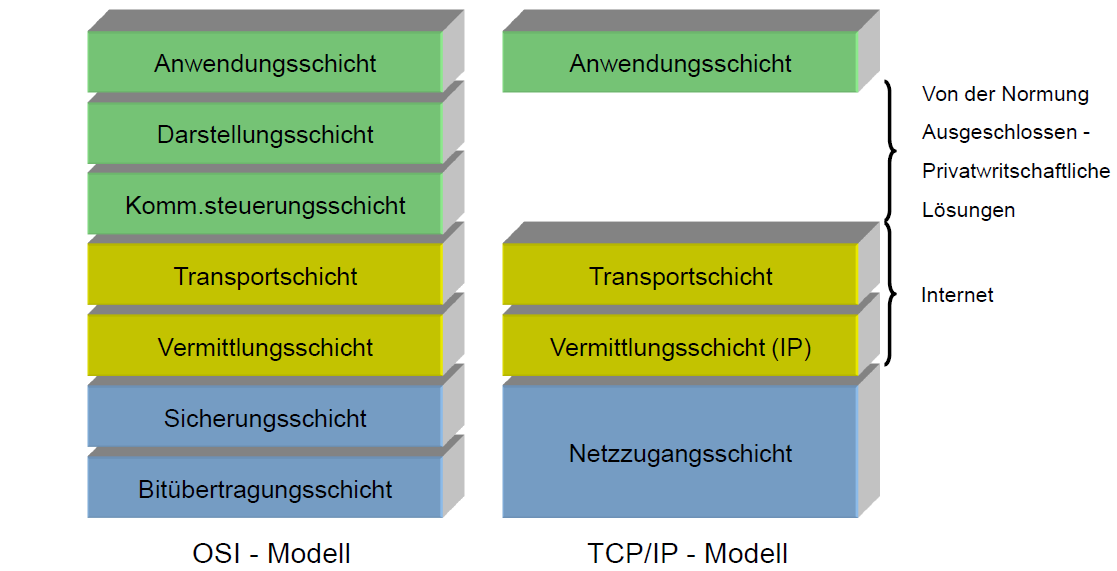
\includegraphics[width = \textwidth]{tcp_ip_model.png}


    \begin{enumerate}[\thesection .1]
        \item{Application Layer}\\\\
        Umfasst alle höherschichtigen Protokolle des TCP/IP-Modells.
        Zu den ersten Protokollen der Verarbeitungsschicht zählen TELNET (für virtuelle Terminals),
        FTP (Dateitransfer) und SMTP (zur Übertragung von E-Mail).
        Im Laufe der Zeit kamen zu den etablierten Protokollen viele weitere Protokolle wie z.B.
        DNS (Domain Name Service) und HTTP (Hypertext Transfer Protocol) hinzu.\\

        \begin{addmargin}[1em]{1em}
            \emph{Protokolle:}
            \begin{enumerate}[$\diamond$]
                \item DNS (Domain Name System) - Umsetzung zwischen Domainnamen und IP-Adressen.\\
                \item DoIP (Diagnostic over IP) - Transportprotokoll für Fahrzeugdiagnose.\\
                \item FTP (File Transfer Protocol) - Dateitransfer.\\
                \item HTTP (Hyper Text Transfer Protocol, WWW)\\
                \item HTTPS - (Hyper Text Transfer Protocol Secure)\\
                \item IMAP (Internet Message Access Protocol) - Zugriff auf E-Mails.\\
                \item IPFIX (Internet Protocol Flow Information Export)\\
                \item L2TP (Layer 2 Tunneling Protocol)\\
                \item LLMNR (Link-local Multicast Name Resolution)\\
                \item NDMP (Network Data Management Protocol)\\
                \item MBS/IP (Multi-purpose Business Security over IP)\\
                \item NNTP (Network News Transfer Protocol) - Diskussionsforen (Usenet)\\
                \item NTP (Network Time Protocol)\\
                \item POP3 (Post Office Protocol, Version 3) - E-Mail Abruf\\
                \item RTP (Real-Time Transport Protocol)\\
                \item SIP (Session Initiation Protocol) - Aufbau, Steuerung und Abbau von
                Kommunikationssitzung (VoIP).\\
                \item SNMP (Simple Network Management Protocol) - Verwaltung von Geräten im Netzwerk.\\
                \item SMTP (Simple Mail Transfer Protocol) - E-Mail Versand.\\
                \item SOCKS (Internet Sockets-Protokoll)\\
                \item SSH (Secure Shell) - verschlüsselter REMOTE TERMINAL\\
                \item Telnet - unverschlüsseltes Login auf entfernten Rechnern.\\
                \item XMPP (Extensible Message and Presence Protocol)\\
                \item Z39.50 - Abfrage von Informationssystemen\\
            \end{enumerate}
        \end{addmargin}

        \item Transport Layer:\\\\
        Ermöglicht wie im OSI-Modell die Kommunikation zwischen Quell- und Zielhost.\\
        Hierzu wurden zwei End-zu-End-Protokolle definiert:

        \begin{addmargin}[1em]{1em}
            - Transmisstion Control Protocol (TCP)
            \begin{addmargin}[1em]{1em}
                TCP ist ein zuverlässiges verbindungsorientiertes Protokoll, durch das
                ein Bytestrom fehlerfrei einem anderen Rechner im Internet übermittelt
                werden kann. Mittels virtuellem Handshake wird sichergestellt, dass die Daten fehlerfrei und
                ganzheitlich transferiert wurden.
            \end{addmargin}
            - User Datagram Protocol (UDP)
            \begin{addmargin}[1em]{1em}
                UDP ist ein unzuverlässiges Protokoll, welches vorwiegend in Client/Server-
                Umgebungen verwendet wird, in denen es in erster Linie nicht um eine sehr genaue,
                sondern schnelle Datenübertragung geht. Durch das ungecheckte Versenden können hierbei
                Datensätze verloren gehen.\\
            \end{addmargin}

            \emph{Protokolle:}
            \begin{enumerate}[$\diamond$]
                \item TCP (Transmission Control Protocol) - Übertragung von Datenströmen
                (verbindungsorientiert, zuverlässig).
                \item UDP (User Datagram Protocol) - Übertragung von Datenpaketen
                (verbindungslos, unzuverlässig, geringer Overhead).
                \item SCTP (Stream Control Transmission Protocol) - Transportprotokoll.
                \item TLS (Transport Layer Security) - Erweiterung von TCP um Verschlüsselung.
                \item DTLS (Datagram Transport Layer Security) - Auf TLS basierendes
                Verschlüsselungsprotokoll, das auch über zustandslose Protokolle wie UDP
                übertragen werden kann.
            \end{enumerate}
        \end{addmargin}

        \item Internet Layer:\\
        Diese Schicht definiert nur ein Protokoll namens IP (Internet Protocol), das alle am Netzwerk
        beteiligten Geräte verstehen können. Sie hat die Aufgabe IP-Pakete richtig zuzustellen. Dabei
        spielt das Routing der Pakete eine wichtige Rolle. Das Internet Control Message Protocol (ICMP)
        ist fester Bestandteil jeder IP-Implementierung und dient zur Übertragung von Diagnose- und
        Fehlerinformation für das Internet Protocol.\\

        \begin{addmargin}[1em]{1em}
            \emph{Protokolle:}
            \begin{enumerate}[$\diamond$]
                \item IP (Internet Protocol) - Datenpalet-Übertragung (verbindungslos)\\
                \item IPsec (Internet Protocol Security) - Sichere Datenpaket-Übertragung (verbindungslos)\\
                \item ICMP (Internet Control Message Protocol) - Kontrollnachrichten (zum Beispiel Fehlermeldungen),
                Teil jeder IP-Implementierung\\
                \item IGRP (Interior Gateway Routin Protocol) - Informationsaustausch zwischen Routern (Distanzvektor)
                (veraltet - ersetzt durch EIGRP)\\
                \item OSPF (Open Shortes Path First) - Informationsaustausch zwischen Routern (Linkzustand) via IP\\
                \item BGP (Border Gateway Protocol) - Informationsaustausch zwischen autonomen Systemen im Internet via TCP\\
                \item RIP (Routing Information Protocol) - Informationsaustausch zwischen Routern vid UDP\\
                \item IGMP (Internet Group Management) - Organisation von Multicast-Gruppen, Bestandteil von IP auf allen Hosts,
                die den Empfang von IP-Multicast unterstützen\\
            \end{enumerate}
        \end{addmargin}

        \item Network Layer:\\\\
        Unterhalb der Internetschicht befindet sich im TCP/IP-Modell eine große Definitionslücke.
        Das Referenzmodell sagt auf dieser Ebene nicht viel aus, was hier passieren soll. Festgelegt ist
        lediglich, dass zur Übermittlung von IP-Paketen ein Host über ein bestimmtes Protokoll an ein Netz
        geschlossen werden muss. Dieses Protokoll ist im TCP/IP-Modell nicht weiter definiert und weicht
        von Netz zu Netz und Host zu Host ab. Dieses Modell macht an dieser Stelle vielmehr Gebrauch von
        bereits vorhandenen PRotokollen, wie z.B. Ethernet (IEE 802.3), Serial Line IP(SLIP), etc.\\

        \begin{addmargin}[1em]{1em}
            \emph{Protokolle:}\\
            \begin{enumerate}[$\diamond$]
                \item Ethernet mit CSMA/CD - Netzwerkstandard IEEE 802.3\\
                \item WLAN - Netzwerkstandard IEEE 802.11\\
                \item PPP - Point-to-Point Protokoll\\
                \item Token Bus - Netzwerkstandard IEEE 802.4\\
                \item Token Ring - Netzwerkstandard IEEE 802.5\\
                \item FDDI - Fiber Distributed Data Interface\\
                \item ARP ( Adress Resolution Protocol) - Adressumsetzung zwischen IP- und Geräteadressen (MAC)\\
                \item RARP ( REverse Adress Resolution Protocol) - Adressumsetzung zwischen Geräte- (MAC) und IP-Adressen
                (veraltet - wird durch BOOTP ersetzt)\\\\
            \end{enumerate}
        \end{addmargin}
    \end{enumerate}

    TCP Three-Way-Handshake:
    \begin{enumerate}
        \item Kontakt mit anderem Computer aufnehmen, indem Nachricht x gesendet wird.
        \item Nun antwortet der Server mit der Sequenz, die er vom Client bekommen hatte,
        jedoch wurde zu dieser Sequenz plus eins dazu gerechnet.
        \item Um Verbindung entgültig aufzubauen, antwortet der Client noch ein letztes mal.\\
    \end{enumerate}
    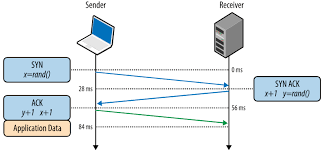
\includegraphics[width=\textwidth]{images.png}

\end{document}